\chapter{Digital image processing} \label{chp:proc}
%
\section{Introduction}
\par
The goal of the digital image processing described below is to identify the air-water surface emphasized by the planar laser induces fluorescence (PLIF) technique.
This image processing assumes that there is a dark region at the top of the image, and that there is a connected bright region across the image at some elevation, or vice-versa. 
While this code has primarily been tested on PLIF images using a laser sheet, it could be applied to many types of fluid flow, e.g. water illuminated by a laser or turbulent aerated flow viewed through a transparent window.
The algorithm described below applies to surfaces which are single valued for any given pixel column.
This is a consequence of the simple surface pixel selection processing. 
%
\section{Algorithm outline}
\par
The air-water surface will be identified by find the uppermost valid local maximum of the image gradient.
Here, the challenge is identifying {\em valid} candidates.
Practical challenges can lead to unwanted imaging artifacts such as reflections, or undesired features such as splash up droplets.
Identifying local maxima allows for interpolating the location of the maxima with simple functions, in this case a quadratic function is chosen.
Interpolation of the maxima reduces the stair-step artifact created by discrete pixel locations.
\par
An algorithm to analyze each image is outlined as follows:
%
\begin{itemize}
	\item Preliminary processing (see \S \ref{sec:prelimprocess})
	\begin{itemize}
		\item Convert to grayscale if needed (see \S \ref{sec:greyscale})
		\item Normalize the image (see \S \ref{sec:normalize})
		\item Median filter the image (see \S \ref{sec:medianfilt})
		\item Denoise the image using non-local means de-noising (see \S \ref{sec:imagedenoising})
		\item Undistort the image if needed (see \S \ref{sec:lensdistortion})
	\end{itemize}
	\item Calculate the magnitude of image gradient with Scharr convolution filter (see \S \ref{sec:gradientoperators})
	\item Select valid maxima of the gradient (see \S \ref{sec:valid-maxima})
	\begin{itemize}
		\item Identify the largest gradient in each column (see \S \ref{sec:column-max})
		\item Identify sufficiently large gradients (see \S \ref{sec:segmentation})
		\item Identify water surface by phase (see \S \ref{sec:phasing})
		\item Identify water surface by shape (see \S \ref{sec:isolation})
		\item Identify all local maxima (see \S \ref{sec:localmaxima})
	\end{itemize}
	\item Identify the uppermost maxima for each column with weighting function (see \S \ref{sec:uppermostcandidate})
	\item Output integer values as surface line
	\item For each surface line location, super-sample the maxima with adjacent intensity values (details in \S \ref{sec:supersample})
	\item Output super-sample adjustment
\end{itemize}
%
Note that, with the exception of the super-sampling method, the algorithm is composed of existing image processing algorithms.
These algorithms were chosen because they are available in commonly available image processing toolboxes, such as OpenCV and its implementations in Python, Matlab, Java, etc.
This means that this algorithm could be easily implemented in the researcher's preferred programming language.
\par
This algorithm is designed to work exclusively in image space with image concepts.
Converting the identified surface line to a physical quantity is discussed in chapter \ref{chp:post}.
The details of each step is discussed in the following sections.
%
\section{Preliminary processing} \label{sec:prelimprocess}
%
\subsection{Grayscale images} \label{sec:greyscale}
\par
In the case of PLIF, color images may be converted to grayscale with a simple weighted average, as the signal is primarily independent of color.
Choosing a grayscale camera that has a higher sensitivity to light (ISO) may be preferred to a color camera.
In some cases color can be useful for segmenting an image, although they are not discussed here.
%
\subsection{Histogram normalization} \label{sec:normalize}
\par
Histogram normalization is used to ensure that bright spots are not too bright, and that dark spots are not too dark.
This helps ensure a uniform intensity gradient across the water surface.
In particular, it helps reduce the impact of `hot-spots' in the laser sheet created by a cylindrical lens or powell lens.
Generally, it makes analysis of the images more robust.
Note that histogram equalization techniques tend to introduce more problems than they solve when applied to PLIF images, so they are not used or discussed in detail.
%
\subsection{Median filter} \label{sec:medianfilt}
\par
For PLIF images of a water surface, a common artifact is the appearance of small particles in the water surface image.
With the exception of turning the laboratory into a clean room, dust is unavoidable.
Such artifacts may be readily mitigated with a median filter.
A median filter is advantageous here because it is edge preserving, e.g. consider a step function with white noise.
In contrast to a low pass filter like a mean filter, the median filter does not move or spread the step.
The edge preserving feature is important because we wish to identify the edge between the air and water in the image.
In addition, a median filter excels at removing isolated peaks, e.g. a delta function with white noise.
The dust particles are both small and highly illuminated in the image, and appear as sudden jump in the water surface.
Accordingly, they may be efficiently removed with a median filter.
Consider the example shown in figure \ref{fig:medianfilt}.
%
\begin{figure}[H]
	\centering
	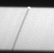
\includegraphics[width=0.45\textwidth]{../images/particle-example-1-original-cropped.png}
	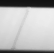
\includegraphics[width=0.45\textwidth]{../images/particle-example-1-median-cropped.png}
	\caption{Small particle removal from the water surface of an example PLIF image.
	Original image shown left, median filtered image shown right.}
	\label{fig:medianfilt}
\end{figure}
%
\subsection{Image de-noising} \label{sec:imagedenoising}
\par
Image de-noising is important for taking a meaningful image gradient.
It is known that gradient operators emphasize white noise, in this case the white noise introduced by the image sensor.
Such noise may produce an artificial gradient when there is not one in the physical signal.
To combat this, a popular method is low pass filtering, because these filters are well established in the signal processing community.
Low pass filtering an image, therefore smoothing sharp edges, before high pass filtering an image in order to emphasize edges is contradictory to the goal presented here.
In addition, there is no reason to assume that the intensity values in an image are dependent on the values near it.
\par
Such observations are the motivation for implementing the non-local means denoising method.
OpenCV implements a version developed by \href{http://www.ipol.im/pub/art/2011/bcm_nlm/}{Buedes et al. (2011)}.
This way images can be denoised while minimizing the smoothing of sharp edges.
If the non-local means denoising method is for some reason not available, consider the denoising properties of a median filter, as shown in figure \ref{fig:medianfilt}.
%
\subsection{Removing lens distortion} \label{sec:lensdistortion}
\par
Lens distortion is removed with the model used in OpenCV ($>4.1.0$).
The model is as follows:
%
\begin{gather*}
	p'' = \frac{p''' - c_p}{f_p} \\
	q'' = \frac{q''' - c_q}{f_q} \\
	r^2 = (p'')^2 + (q'')^2 \\
	p' = p'' \left( 1 + k_1 r^2 + k_2 r^4 + k_3 r^6 \right) + 2p_1 p'' q'' + p_2(r^2 + 2 p''^2) \\
	q' = q'' \left( 1 + k_1 r^2 + k_2 r^4 + k_3 r^6 \right) + p_1 (r^2 + 2 q''^2) + 2 p_2 p'' q'' \\
	p = f_p p' + c_p \\
	q = f_q q' + c_q
\end{gather*}
%
where $I(p''',q''')$ describes the original image, $p'''$ and $q'''$ are the integer pixel coordinates of the original image, $k_1, k_2, k_3, p_1, p_2$ are lens distortion parameters determined in advance, and $f_p, f_q, c_p, c_q$ are lens intrinsic parameters determined in advance.
At this stage $p$ and $q$ are not integer values, and so the image must be re sampled onto an integer grid as a standard image.
Typically, this is done by interpolating cubic splines to the image, however the exact method depends on the implementation used.
The undistorted image is now ready for analysis.
%
\subsection{Order of pre-processing steps}
\par
The order in which the pre-processing steps is not critical.
A comparison between three different orders of application of the sub-steps shows qualitatively similar results.
The image noise is typically within $\pm 0.1$ pixels, and the spike from the small particle is reduced to $\sim 0.3$ pixels, regardless of the order of application.
%
\begin{figure}[H]
	\centering
	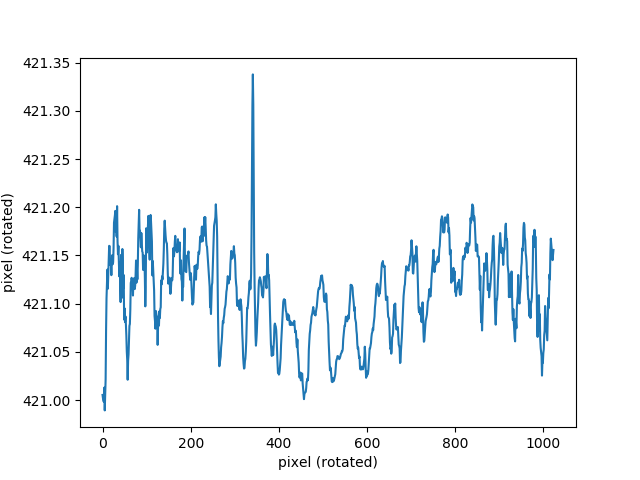
\includegraphics[width=0.3\textwidth]{../images/particle-example-1-median-normalized-denoised.png}
	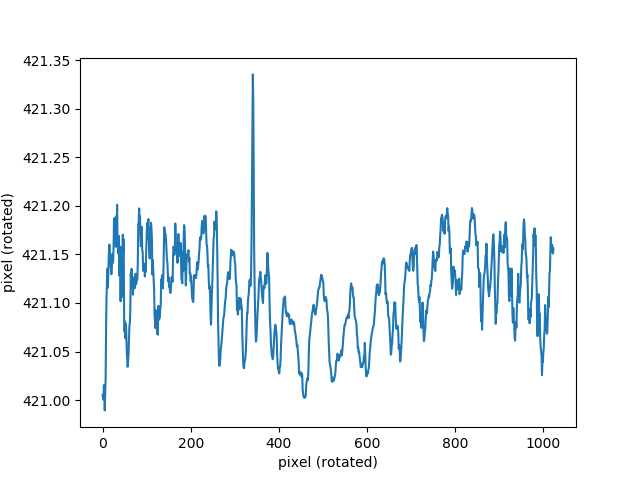
\includegraphics[width=0.3\textwidth]{../images/particle-example-1-normalized-median-denoised.png}
	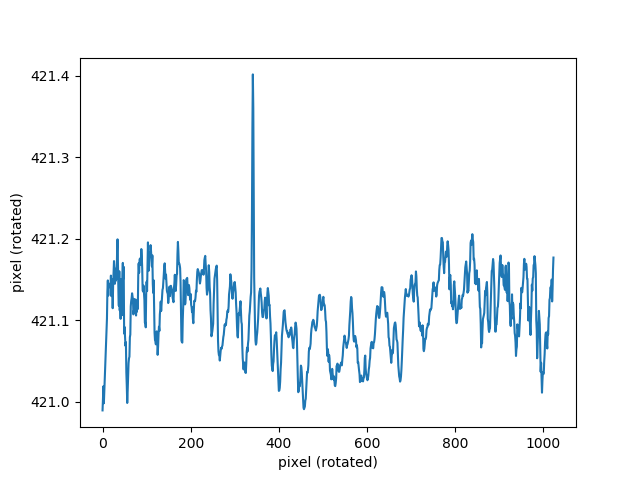
\includegraphics[width=0.3\textwidth]{../images/particle-example-1-denoised-median-normalized.png}
	\caption{Comparison of order of preprocessing techiques. Left) median filter, normalization, then denoising. Center) normalization, median filter, then denoising. Right) denoising, median filter, then normalization. Data shown is from processing the same images shown in figure \ref{fig:medianfilt}.}
\end{figure}
%
\section{Gradient operators} \label{sec:gradientoperators}
\par
Common convolution filters for estimating the image gradient are the central differences, Sobel, and Scharr filters, which are:
%
\begin{gather*}
G_{x,central} = 
\begin{bmatrix}
1, 0, -1
\end{bmatrix}
\text{ ; }
G_{y,central} = 
\begin{bmatrix}
1 \\ 0 \\ -1
\end{bmatrix}
\text{ ; } \\
G_{x,sobel} = 
\begin{bmatrix}
1 & 0 & -1 \\
2 & 0 & -2 \\
1 & 0 & -1
\end{bmatrix}
\text{ ; }
G_{y,sobel} = 
\begin{bmatrix}
1 & 2 & 1 \\
0 & 0 & 0 \\
-1 & -2 & -1
\end{bmatrix}
\text{ ; } \\
G_{x,scharr} = 
\begin{bmatrix}
3 & 0 & -3 \\
10 & 0 & -10 \\
3 & 0 & -3
\end{bmatrix}
\text{ ; }
G_{y,scharr} = 
\begin{bmatrix}
3 & 10 & 3 \\
0 & 0 & 0 \\
-3 & -10 & -3
\end{bmatrix}
\text{ ; }
\end{gather*}
%
where each kernel must be normalized such that the sum of its parts is one.
Each kernel designed to be computation efficient and valid estimates of the gradient in their own way.
I have struggled to find comprehensive work on the details of each, however, Scharr's filter is the result of his PhD thesis (evidently, but I can't read German).
Both the Sobel and Scharr filter are more robust to noise than the central differences filter.
Scharr's filter is chosen without a proper reason over the sobel filter.
The gradient in both the x and y direction are estimated, then the magnitude and phase are taken in the usual way.
%
\section{Finding valid maxima} \label{sec:valid-maxima}
\par
In order to find the first {\em valid} local maximum of the gradient, gradients which are suitably small to be considered background noise must be ignored.
Selecting valid local maxima can be achieved in a variety of ways.

\subsection{Column maxima} \label{sec:column-max}
\par
The simplest and fastest method to find the water surface is to identify the largest gradient value in each pixel column.
This method only works with careful physical preparation and may be invalided by unexpected imaging artifacts.
The results are guaranteed to be a maxima or plateau edge, so no further refinement is needed.
Use this if it works.

\subsection{Segmentation} \label{sec:segmentation}
\par

Standard segmentation methods can be used to find the water surface.
In figure \ref{fig:segmentation-gradient}, an image gradient is segmented using both Otsu thresholding and kmeans-clustering.
It can bee seen that kmeans-clustering with two clusters is analogous to Otsu thresholding, in this case.
In contrast, utilizing multiple clusters allows for fine control of the segmentation.
Utilizing too few clusters may not properly identify the connectivity of the surface, as shown in case of two cluster.
Utilizing too many clusters may overly connect the surface, as shown in the case of four clusters.
In this case, three clusters provides a sweet spot where the entire surface is identified as a single connected group in addition to being isolated from the lower surface.
Additionally, the number of clusters is a adjustable parameter and can be chosen based on the data being analyzed.
%
\begin{figure}[H]
	\centering
	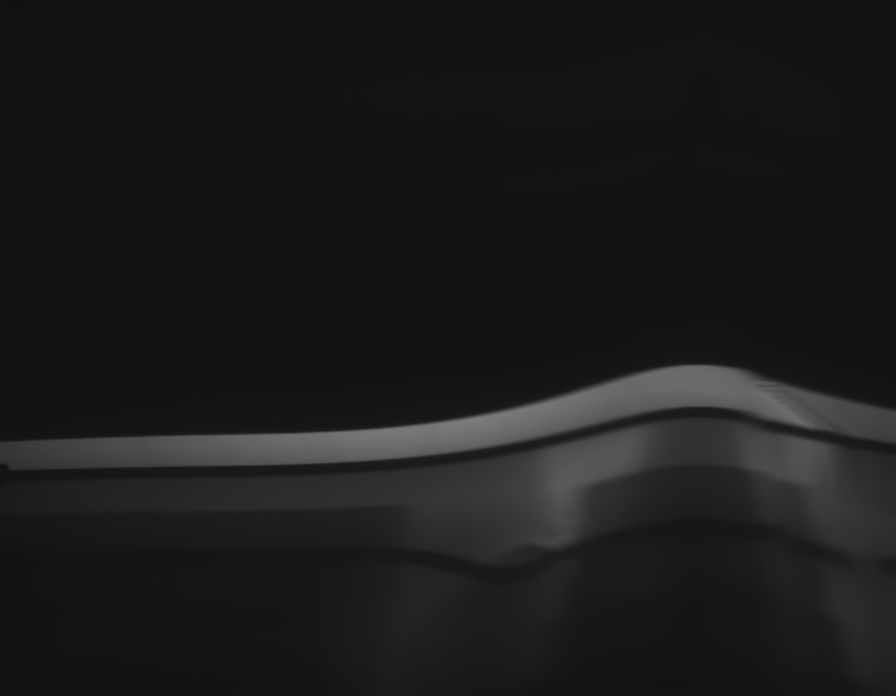
\includegraphics[width=0.30\textwidth]{../images/exp-original.png}
	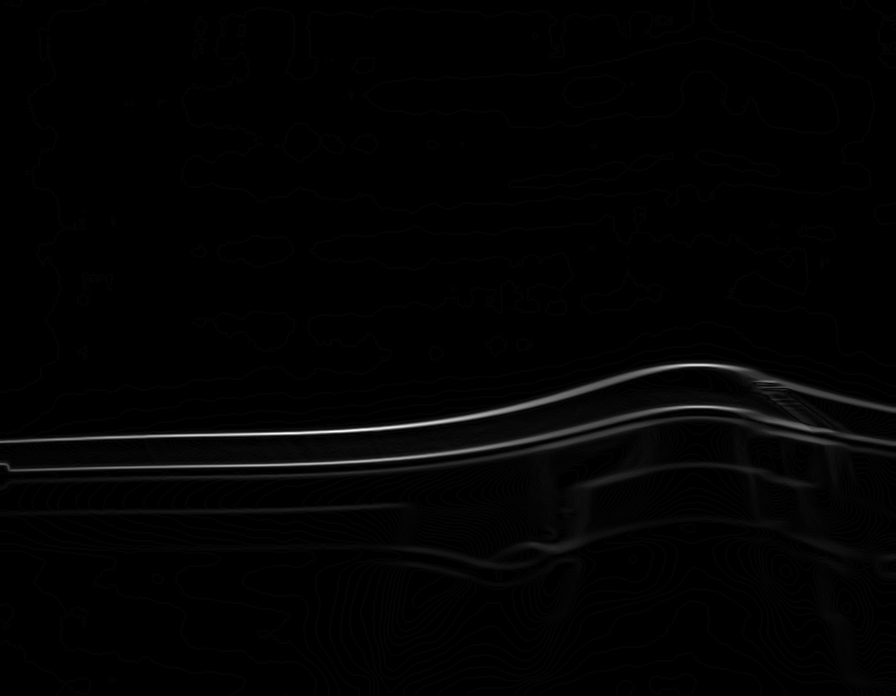
\includegraphics[width=0.30\textwidth]{../images/exp-gradient.png}
	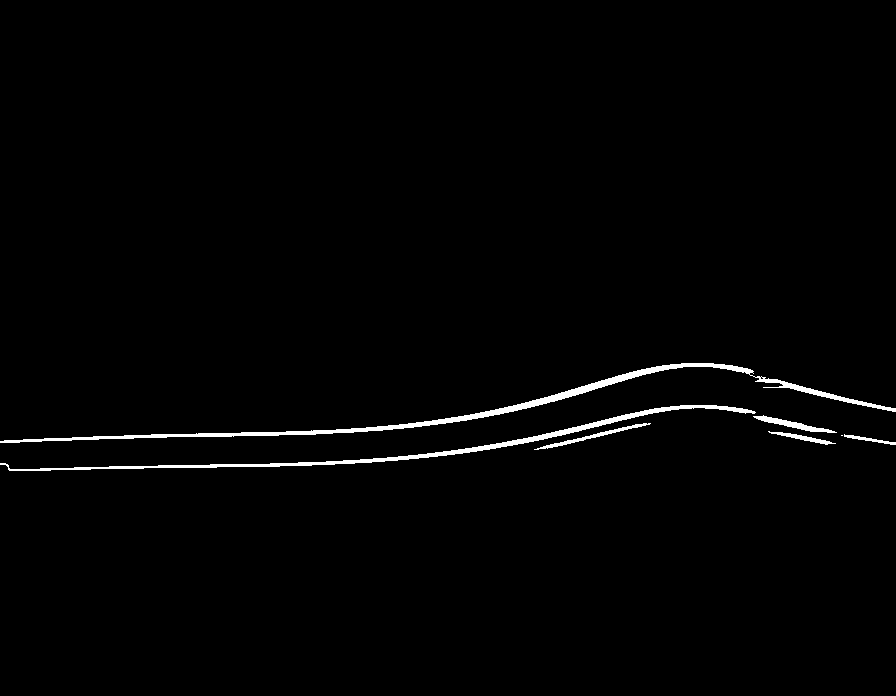
\includegraphics[width=0.30\textwidth]{../images/exp-mask-otsu.png}
	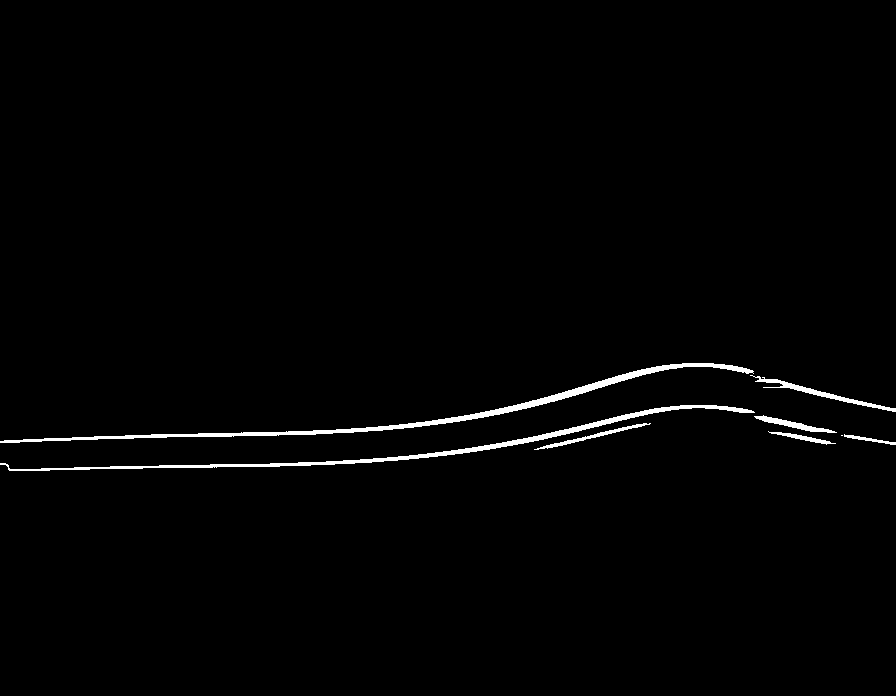
\includegraphics[width=0.30\textwidth]{../images/exp-mask-kmeans-2.png}
	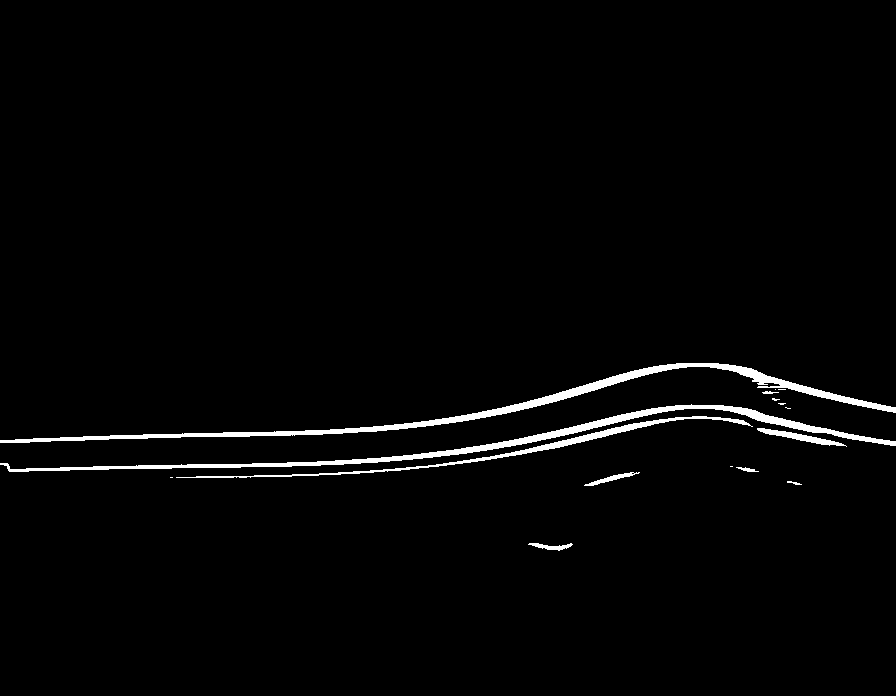
\includegraphics[width=0.30\textwidth]{../images/exp-mask-kmeans-3.png}
	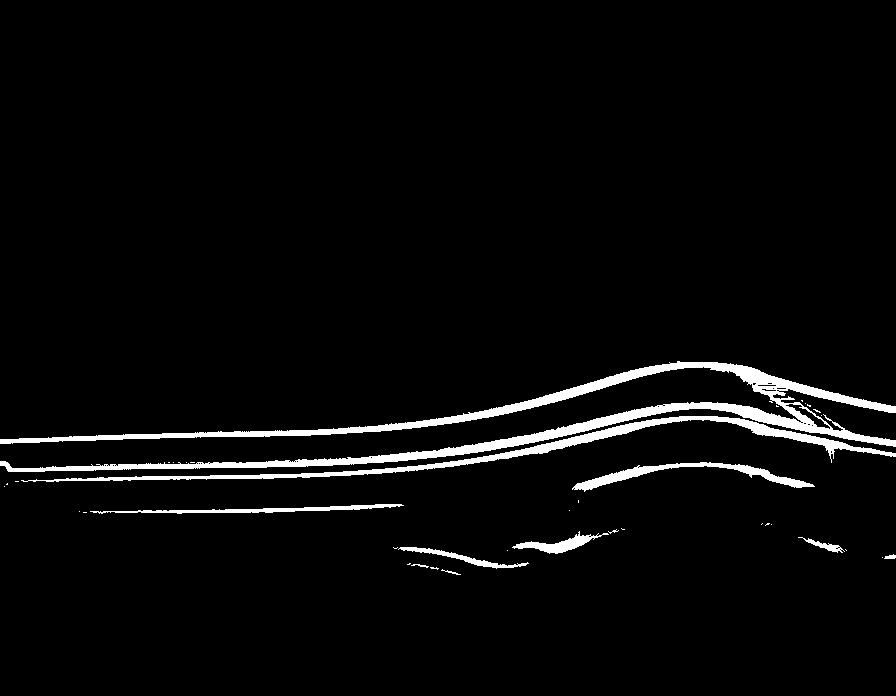
\includegraphics[width=0.30\textwidth]{../images/exp-mask-kmeans-4.png}
	\caption{Segmentation of the gradient using a variety of methods. In order from top left to bottom right: First, the original image. Second, the image gradient. Third, the gradient is segmented using otsu thresholding. Fourth, the image is segmented using kmeans clustering with two clusters. Fifth, the image is segmented using kmeans clustering with three clusters. Sixth, the image is segmented using kmeans clustering with four clusters.}
	\label{fig:segmentation-gradient}
\end{figure}
%
\subsection{Gradient phase (optional)} \label{sec:phasing}
\par
Selecting gradient values by phase may be helpful if the water surface is relatively uniform.
Clustering phase values into a low and high category allows water surfaces to be identified along a uniform edge, e.g. the upper and lower parts of an illuminated sheet.
This can also be helpful where the water surface changes rapidly in a small region (e.g. wave breaking) when used in conjunction with a connected water surface as in \S \ref{sec:isolation}.
Separating by phase may lead to misleading results when the water surface is very steep, e.g. the meniscus effect near a vertical wall.

\subsection{Connected water surface (optional)} \label{sec:isolation}
\par
It may be the goal to identify only a connected surface and remove any imaging artifacts or splash up that might identify a disconnected surface.
To do this, first recognize that connectivity for binary images are easily analyzed for connectivity.
Accordingly, the image mask created by finding locations where the image gradient is sufficiently large can be analyzed for connectivity.
In the simplest case, the uppermost connected surface that spans the entire image may be used to identify the water surface.
However, in some cases, the illuminated water surface does not span the entire image.
This can lead to false positives if the widest water surface is the incorrect one (e.g. the bottom surface of a wave tank).
Use the phase of the gradient as discussed in \S \ref{sec:phasing} in addition to the shape to ensure the correct water surface is chosen.
%
\subsection{Identifying Local Maxima \& Plateaus} \label{sec:localmaxima}
\par
Local maxima are found by comparing the gradient to itself after dilation.
Any pixel that has the same value before and after dilation is a local maxima or plateau.
The dilation kernel used is:
%
\begin{gather*}
K = 
\begin{bmatrix}
1 \\
0 \\
1
\end{bmatrix}
\text{ ; }
\end{gather*}
%
such that local value must be greater than or equal to the value above and below itself.
This definition of local maxima is used for simplicity, and local maxima need only be greater than or equal to the values above and below itself to implement the super-sampling method discussed in section \ref{sec:supersample}.
\par
This method can be expanded to find local maxima and plateaus in a larger region by expanding the kernel.
For example, if the kernel was:
%
\begin{gather*}
K = 
\begin{bmatrix}
1 \\
1 \\
0 \\
1 \\
1
\end{bmatrix}
\text{ ; }
\end{gather*}
%
then the local value must be greater than the values two above and below itself, as well.
In the application of PLIF, maxima in the vertical direction are of interest, and so only values in the column are compared, but this method could be extended to include information in adjacent columns.
%
\section{Identifying the uppermost valid candidate} \label{sec:uppermostcandidate}
%
In order to select the uppermost valid surface candidate in each column, recognize that identified candidates mask have an intensity value of 1 at each location.
Then, the mask can be multiplied by a weighted image which has the largest value at the top of the image, and decreases to 1 at the bottom.
Then, when the images are multiplied together element-wise, the location with the largest intensity value is also the uppermost valid candidate in the column.
The location of this candidate can be identified using a sorting algorithm which returns the index location of the largest value in each column.
\par
Note that there must be a local maximum in {\em every} column for this to work, as most sorting algorithms return a random value if all values are equal in the group.
This limitation can be avoided by returning an invalid value (-1, NaN, etc.) when there is no maximum in the column.
%
\section{Stair step removal in gradient method} \label{sec:supersample}
%
In order to reduce the stair step artifact resulting from digital imaging, the gradient intensity will be interpolated with a quadratic function.
This can be achieved near the identified local maximum using the adjacent points to fit a quadratic.
Then, the maxima of that parabola can be identified analytically.
A quadratic function is chosen because it has a simple notion of concavity.
\par
The intensity values in the column of the image are fit with a quadratic function.
Accordingly, it has values and local maxima defined by:
%
\begin{gather}
I(x) = ax^2 + bx + c \\
x_{max} = \frac{-b}{2 a}
\end{gather}
%
The problem is posed locally by choosing three points at $x=-1$, $x=0$, and $x=1$ such that the coefficients a, b, and c may be found by solving the system of equations:
%
\begin{gather}
I_{j-1} = a - b + c \\
I_{j} = c \\
I_{j+1} = a + b + c
\end{gather}
%
The system can be solved by noting $c=I_j$ then solving for a and be in terms of $I_{j+1}$, $I_{j}$, and $I_{j-1}$:
%
\begin{gather}
I_{j-1} = a - b + I_{j} \\
I_{j+1} = a + b + I_{j} \\
a = I_{j-1} + b - I_{j} = I_{j+1} - b - I_{j} \\
b = \frac{1}{2} \left( I_{j+1} - I_{j-1} \right) \\
a = I_{j-1} + \frac{1}{2} \left( I_{j+1} - I_{j-1} \right) - I_{j}
\end{gather}
%
such that the local maxima of the parabola, interpreted as an adjustment to the local maxima identified in previous analysis, can be found:
%
\begin{gather}
\Delta x = \frac{-b}{2 a} = \frac{- \frac{1}{2} \left( I_{j+1} - I_{j-1} \right)}{2 I_{j-1} + I_{j+1} - I_{j-1} - 2 I_{j}} = \frac{I_{j-1} - I_{j+1}}{2 I_{j-1} + 2 I_{j+1} - 4 I_{j}}
\end{gather}
%
This has the advantage of being easy to implement to an arbitrary precision.
As long as $I_j$ is a local maxima, the adjustment will always be between $-\frac{1}{2} < \Delta x < \frac{1}{2}$.
In the cases where $I_j$ is a plateau edge, e.g. $I_j = I_{j+1}$, then $\Delta x = \frac{1}{2}$ ()the location selected is between the two largest values).